%%
%% Thèse manuscrit 
%% 
%%%%%%%%%%%%%%%%%%%%%%%%%%%%%%%%%%%%%%%%%
%           Initialisation				%
%%%%%%%%%%%%%%%%%%%%%%%%%%%%%%%%%%%%%%%%%


\pdfobjcompresslevel 0
\documentclass[a4paper, 12pt]{report}


%
%%\usepackage{comment} % Permet de compiler sans les figures et sans les tables
%%\excludecomment{figure}
%%\let\endfigure\relax
%%\excludecomment{table}
%%\let\endtable\relax

%\usepackage{refcheck} %permet de voir les refs du bib non cit�es

\setlength{\parindent}{0pt} %get rid of indentation in the article
\usepackage{etoolbox} % prevent a Patching '\begin' failed! see https://tex.stackexchange.com/questions/128938/package-etoolbox-warning-patching-begin-failed
%\usepackage{natbib} % pour bibtex \citep (parenthetical) et \citet (textual) (sinon seul \cite marche) a loader avant babel
\usepackage[semicolon,round,sort&compress,sectionbib]{natbib}  %
\usepackage{chapterbib}      
\usepackage[english, french]{babel} %Fran�ais à loader avant caption
\usepackage[T1]{fontenc}

  \usepackage{adjustbox}
\usepackage[affil-it]{authblk} %for affiliation
\usepackage{afterpage} % To include blanck page with command \afterpage{\blankpage}
\usepackage{appendix}

\usepackage{array} %pour les tableaux
\usepackage{amsmath, amssymb} %american mathematical society math style and symbols (amssymb)
\usepackage{amsthm}
\usepackage{blindtext}
\usepackage{booktabs}
\usepackage{breqn} % allow to use dmath environment (automatic break for equations, etc) 
\usepackage{caption} % Needed to jump line in figures titles (caption).
%\usepackage{commath} sais pas pourquoi �a marche pas si je charge �a plante !

\usepackage{dirtytalk} % quote stuff with \say{the text to quote}
\usepackage{empheq} %
\usepackage[official]{eurosym}  %type \euro{} to print a euro
\usepackage{float} % for firgure placement with H option
\usepackage{fancybox}

  \usepackage[top=2cm, bottom=2cm, left=2.5cm, right=2.5cm]{geometry}
  \usepackage[top=2cm, bottom=2cm, left=2.5cm, right=2.5cm]{geometry}
\usepackage{graphicx} %pour ins�rer des images.
 \usepackage[hyperindex=true,
 		     colorlinks=true, 
		     urlcolor=blue,
		     citecolor    = blue, %Couleur des citations (biblio)
    		     linkcolor    = blue, %Couleur des équations. Apparemment, cela sert aussi pour théoreme, Lemme...
 					 ]{hyperref} %permet de mettre des hyper liens (le package url le fait tout seul ? la base)

\usepackage{import}					 



\usepackage{pdflscape}
\usepackage{pdfpages} %allow to select which pdf pages to compile \includepdf[pages={12-15,23,45-49}]{main.pdf} 
\usepackage{spverbatim}
\usepackage{lmodern}%change un peu les lettres pour un truc plus cool, marche peut �tre un peu mieux avec les accents v�rifier � l'occaz
\usepackage{mathrsfs} % allows $\mathscr{ABC}$ to work
\usepackage{setspace} % permet de d�terminer une largeur d'interligne
\usepackage{tikz} % draw graphs
\usetikzlibrary{trees,shapes,snakes}
  \usepackage{subcaption} % to use with subfigures
\usepackage{skull}
\usepackage{url}
\usepackage{verbatim} %Pour ins�rer du code informatique

\usepackage{fancyvrb}
\usepackage{fvextra}

\usepackage{array} %one of the two needed to use thead to break line in tabular
\usepackage{makecell} %one of the two needed to use thead to break line in tabular

\DeclareUnicodeCharacter{20AC}{\euro{}}
\DeclareUnicodeCharacter{2212}{-}
\DeclareUnicodeCharacter{300}{`}
\DeclareUnicodeCharacter{301}{'}

  \newcommand{\hdrule}{\midrule[\heavyrulewidth]}

\newsavebox{\mybox}

\newcommand{\raisedshadowbox}[1]{%
\sbox\mybox{\shadowbox{#1}}%
\raisebox{-0.5\ht\mybox-0.5\shadowsize+0.6ex}{\usebox\mybox}%
}
%%%%%
\providecommand{\tightlist}{%
  \setlength{\itemsep}{0pt}\setlength{\parskip}{0pt}}


\bibliographystyle{chicagoa}


%%%%%%%%%%%%%%%%
%%%Fin biblio %%%%%%%%



%%%%Elispse in tables%%%%%%
\usepackage{tikz}
\usetikzlibrary{fit,shapes.misc}
\newcommand\marktopleft[1]{%
    \tikz[overlay,remember picture] 
        \node (marker-#1-a) at (0,-1ex) {};%
}
\newcommand\markElipseBottomright[1]{%
    \tikz[overlay,remember picture] 
        \node (marker-#1-b) at (0.2,0.3) {};%
    \tikz[overlay,remember picture,thick,dashed,inner sep=3pt]
        \node[draw, ellipse,fit=(marker-#1-a.center) (marker-#1-b.center)] {};%
}
%%%%End Elispse in tables%%%%%%






%%%%Squares in tables%%%%%%
\newcommand\markRectangletopleft[1]{%
    \tikz[overlay,remember picture] 
        \node (marker-#1-a) at (0,1.5ex) {};%
}
\newcommand\markRectanglebottomright[1]{%
    \tikz[overlay,remember picture] 
        \node (marker-#1-b) at (0,0) {};%
    \tikz[overlay,remember picture,thick,dashed,inner sep=3pt]
        \node[draw,rounded rectangle,fit=(marker-#1-a.center) (marker-#1-b.center)] {};%
}
%%%%Squares Circles in tables%%%%%%


\newcommand\blankpage{%
    \null
    \thispagestyle{empty}%
    \addtocounter{page}{-1}%
    \newpage}




\DeclareMathOperator\erf{erf}


\providecommand{\U}[1]{\protect\rule{.1in}{.1in}}
%EndMSIPreambleData
\newtheorem{theorem}{Theorem}
\newtheorem{acknowledgement}[theorem]{Acknowledgement}
\newtheorem{algorithm}[theorem]{Algorithm}
\newtheorem{axiom}[theorem]{Axiom}
\newtheorem{case}[theorem]{Case}
\newtheorem{claim}[theorem]{Claim}
\newtheorem{conclusion}[theorem]{Conclusion}
%\newtheorem{condition}[theorem]{Condition}
\newtheorem{conjecture}[theorem]{Conjecture}
\newtheorem{corollary}[theorem]{Corollary}
\newtheorem{criterion}[theorem]{Criterion}
\newtheorem{definition}[theorem]{Definition}
\newtheorem{example}[theorem]{Example}
\newtheorem{exercise}[theorem]{Exercise}
\newtheorem{lemma}[theorem]{Lemma}
\newtheorem{notation}[theorem]{Notation}
\newtheorem{problem}[theorem]{Problem}
\newtheorem{proposition}[theorem]{Proposition}
\newtheorem{remark}[theorem]{Remark}
\newtheorem{solution}[theorem]{Solution}
\newtheorem{summary}[theorem]{Summary}
%\newenvironment{proof}[1][Proof]{\noindent\textbf{#1.} }{\ \rule{0.5em}{0.5em}}



\usepackage{fancyhdr}

\usepackage{minitoc} % table of contents should be loaded after hyperef and other packages
\usepackage{silence}


%%%%% Mute minitoc warnings see https://tex.stackexchange.com/questions/166910/what-are-these-warnings-for-minitoc-package
\WarningFilter{minitoc(hints)}{W0023}
\WarningFilter{minitoc(hints)}{W0024}
\WarningFilter{minitoc(hints)}{W0028}
\WarningFilter{minitoc(hints)}{W0030}
\WarningFilter{blindtext}{} % this takes care of the `blindtext` messages

\usepackage{grffile}

\graphicspath{{}}

\frenchbsetup{ShowOptions} 

\Urlmuskip=0mu  plus 10mu  %Solver Overfull \hbox for url links (see https://tex.stackexchange.com/questions/339682/how-to-really-solve-the-problem-of-underfull-hbox-when-typesetting-url-in-f)
%%%%%%%%%%%%%%%%%%%%%%%%%%%%%%%%%%%%%%%%
%           Commandes perso            %
%%%%%%%%%%%%%%%%%%%%%%%%%%%%%%%%%%%%%%%%

\newcommand{\alp}{\texorpdfstring{\ensuremath{\upalpha}\xspace}{alpha }}
\newcommand{\bet}{\texorpdfstring{\ensuremath{\upbeta}\xspace}{b\'{e}ta }}
\newcommand{\alpbet}{\texorpdfstring{\ensuremath{\upalpha-\upbeta}\xspace}{alpha-b\'{e}ta}}
\newcommand{\alpt}{\ensuremath{\alpha_2}\xspace}
\newcommand{\strt}{\gls{strt}\xspace}


% Divers
\newcommand{\FRA}{$\text{FRA}$ }
\newcommand{\MR}{$\text{MR}$ }


% Tenseur des déformation cylindrique
\newcommand{\epsrr}{\ensuremath{\varepsilon_{rr}}\xspace}
\newcommand{\epstt}{\ensuremath{\varepsilon_{\theta\theta}}\xspace}
\newcommand{\epszz}{\ensuremath{\varepsilon_{zz}}\xspace}
\newcommand{\epsrt}{\ensuremath{\varepsilon_{r\theta}}\xspace}
\newcommand{\epstz}{\ensuremath{\varepsilon_{\theta z}}\xspace}
\newcommand{\epszr}{\ensuremath{\varepsilon_{zr}}\xspace}

\newcommand{\matlab}{\textsc{Matlab}\texttrademark\xspace}



%% Figures centrées, et en position 'here, top, bottom or page'
\newenvironment{figureth}{
		\begin{figure}[htbp]
			\centering
	}{
		\end{figure}
		}
		
		
%% Tableaux centrés, et en position 'here, top, bottom or page'
\newenvironment{tableth}{
		\begin{table}[htbp]
			\centering
			%\rowcolors{1}{coleurtableau}{coleurtableau}
	}{
		\end{table}
		}

%% Sous-figures centrées, en position 'top'		
\newenvironment{subfigureth}[1]{
	\begin{subfigure}[t]{#1}
	\centering
}{
	\end{subfigure}
}

\newcommand{\citationChap}[2]{
	\epigraph{\og \textit{#1} \fg{}}{#2}
}

% Macro pour créer une figure (avec notes optionnelles) dans le corps du texte %
\newenvironment{fig}[4][1]{
\begin{figure}[!ht]
	\begin{center}
	\begin{minipage}{14cm}
		\caption{#2}
	\end{minipage}
	\end{center}
	\begin{center}
	\begin{minipage}{#1}
	\begin{center}#3
	\end{center}
	\end{minipage}
	\if!#4!\empty \else \\
	\begin{scriptsize}
	\begin{minipage}{#1}\vspace{0.2cm} \par #4
	\end{minipage}
	\end{scriptsize} \fi }
	{\end{center}
\end{figure}}

% Macro d'inclusion de graphiques pdf %
\newcommand{\graphique}[2][1]{\begin{minipage}{\linewidth}\begin{center}\includegraphics[width=#1\linewidth,clip]{Figures/#2}\end{center}\end{minipage}}


% Macro pour créer un tableau (avec notes optionnelles) %
\newenvironment{tab}[4][1]
{\def\TMP{#3}\newdimen\TMPsize\settowidth{\TMPsize}{\TMP}
\begin{table}[!ht]
\begin{center}
\begin{minipage}{14cm}
\caption{#2}
\end{minipage}
\end{center}
\begin{center}
\begin{minipage}{#1}
\resizebox{\textwidth}{!}{#3}
\end{minipage}
\if!#4!\empty \else \\
\begin{scriptsize}
\begin{minipage}{#1}\vspace{0.2cm} \par #4
\end{minipage}
\end{scriptsize} \fi }
{\end{center}
\end{table}}

%%%%% Pour prendre en compte les commandes \tightlist issues des conversions makdown à Latex de pandoc
\providecommand{\tightlist}{%
  \setlength{\itemsep}{0pt}\setlength{\parskip}{0pt}}	% Commandes et environnements perso
\usepackage{fancyhdr}
\newcommand{\isEmbedded}{true}


%%%%%%%% Liste des fichiers à compiler %%%%%%%%
% Par default : tous
%\includeonly{Introduction}

\usepackage{appendix}  %Pour les appendix
\usepackage{chngcntr}
\usepackage{etoolbox}


\AtBeginEnvironment{subappendices}{%
\chapter*{Appendix}
\addcontentsline{toc}{chapter}{Appendices}
\counterwithin{figure}{section}
\counterwithin{table}{section}
}
\begin{document}

\hypersetup{	
    pdfauthor={Adrien Pacifico},
    pdfsubject={Manuscrit thèse},
    pdftitle={XX},
}


\doparttoc[c]
\mtcsetfeature{parttoc}{open}{\vspace{-2cm}}
\tightmtctrue
\setcounter{parttocdepth}{2}

%%%%%%%%%%%%%%%%% Préambule %%%%%%%%%%%%%%%%%
 
\pagenumbering{roman}
%l'EHESS ne veut que sa page de couverture violette
%\includefrom{../0_Preambule/}{Preambule_ehess}	
\selectlanguage{french} 
\includefrom{./00_preambule/}{Preambule}	

\cleardoublepage

% %%%%%%%%%%%%%%%%% Introduction %%%%%%%%%%%%%%%%%
 \pagenumbering{arabic}
% % Introduction 
 \renewcommand*\thesection{\arabic{section}}

\includefrom{./01_Introduction/}{introduction}


\chapter[Monthly Income Tax Frequency:Theoretical and Empirical Investigations]{Monthly Income Tax Frequency:\\
Theoretical and Empirical Investigations\raisebox{.3\baselineskip}{\normalsize\footnotemark}}
\footnotetext{This chapter is a collaboration with Olivier Bargain \& Alain Trannoy}
\selectlanguage{english}
\graphicspath{{./1_Tax_Frequency/figures/}}
\includefrom{./1_Tax_Frequency/}{tax_frequency}	


\chapter[A Direct Measure of Inefficiency within Couples]{A Direct Measure of Inefficiency within Couples:
Tax Optimization in French cohabiting couples\raisebox{.3\baselineskip}{\normalsize\footnotemark}}
\footnotetext{This chapter is a collaboration with Olivier Bargain, Damien Echevin  \& Nicolas Moreau}
\selectlanguage{english}
\graphicspath{{./2_Cohabiting_couples/figures/}}
\includefrom{./2_Cohabiting_couples/}{cohabiting_couples}	

% \chapter{hello
\chapter{{\sc Rich households taxable income and lowerings of the child tax
break ceiling: \\ \Large{A French natural experiment.}}}
\selectlanguage{english}
\graphicspath{{./3_QF_lowering/figures/}}
\includefrom{./3_QF_lowering/}{qf_lowering}	
\includefrom{./Divers/softwares/}{softwares}


%
% \fancyhead{}
% \fancyhead[LE]{\textsc{Main introduction}}
% \fancyhead[RO]{\textsc{Main introduction}}
% \includefrom{../1_Introduction/}{introduction}	
% \fancyhead{}

% \setcounter{chapter}{0}



% %%%%%%%%%%%%%%%%% Partie I %%%%%%%%%%%%%%%%%
% \part[\textsc{Your title of part 1}]
% {\textsc{Your title of part 1}}
% 	\fancyhead[LE]{\textsc{Partie I -- Entête de la partie I}} % Entete partie I

% This part is dedicated to the study of the redistributive impact of the French tax-and-benefit system. The main focus of this part is methodological. It consists in presenting the microsimulation technique used for describing the distributional impact of taxation. 

% Chapter~\ref{chapter1} offers an introduction to the microsimulation method and its contribution to the analyses of the redistributive impact of the tax-and-benefit system. For that purpose, I present a microsimulation model of French tax revenues. This model simulates French tax revenues based on a representative sample of the French population. Its first feature is to provide a detailed distribution of top incomes, some of them being imputed. Secondly, the aggregated individual level characteristics are consistent with national account. The model decomposes at the micro-level the whole scope of tax revenues as defined in the national accounts. This enables to provide detailed redistributive analyses of fiscal reforms, including at the top at the income distribution. The chapter discusses as well the limitation of this approach. Indeed, the underlying incidence assumption as well as the absence of consistency between aggregate sources can affect the results. 

% Chapter~\ref{chapter2} provides an example of policy evaluation relying on microsimulation. 
% It analyses the impact of the post-2008 crisis political responses in France. It encompasses both a macro and a micro analyses, relying on the study of documents associated to the Budget Laws and on the microsimulation model. 
% The study reveals that the decrease in public spending was used as the main political channel of response although no systemic reform of the organization of spending was achieved.\\

% \mtcsettitle{parttoc}{\textsc{Outline of part I}}
% \noptcrule  
% %\parttoc

% %%% Chapitre 1 %%%
% 	\selectlanguage{french} 
% 	\fancyhead{}
% 	\fancyhead[LE]{\textsc{Partie I -- Entête de la partie I}} % Entete partie I
% 	\fancyhead[RO]{\textsc{Chapitre 1-- Entête du chaptitre 1}} % Entete chapitre 1



% 	\fancyhead{}
% %%% Chapitre 2 %%%	
% \selectlanguage{english} 
% 	\fancyhead{}
% 	\fancyhead[LE]{\textsc{Part I -- The short title of part I}} % Entete partie I
% 	\fancyhead[RO]{\textsc{Chapter 2-- The title of chapter 2}} % Entete chapitre 2
% 	\includefrom{../2_Partie1/2_chapter2/}{chapter2}
% 	\fancyhead{}
		

% \renewcommand{\partname}{}
% 	\part*{}

% %%%%%%%%%%%%%%%%% Partie II %%%%%%%%%%%%%%%%%
% \selectlanguage{english} 
% %\part{\textsc{Primary inequality and redistribution through employer Social Security contributions: France 1976-2010}} 
% \part[\textsc{Your title of part II}]{\textsc{Your title of part II}}

% \mtcsettitle{parttoc}{\textsc{Outline of part II}}
% \noptcrule  
% %\parttoc

% This second part focuses on the taxation of labour incomes and rests upon the methodology presented in the first part. The questions and the methods tackled by this part are at the intersection of the public finance and the labour economics literature. Chapter~\ref{chapter3} studies the overall wage distribution whereas chapter~\ref{chapter4} focuses on the very top wages (top 0.003\% of the distribution, about 1500 individuals). These two chapters are complementary in the sense that the first one focuses on the long term evolution of taxation and labour inequality of the broad wage distribution whereas the second chapter is centred on top 0.01\% of the same distribution.\\


% 	%%% Chapitre 3 %%%
% 	\fancyhead{}
% 	\fancyhead[LE]{\textsc{Part II -- The short title of part II}} % Entete partie II
% 	\fancyhead[RO]{\textsc{Chapter 3-- The title of chapter 3}} % Entete chapitre 3
% 	\includefrom{../3_Partie2/1_chapter3/}{chapter3}	
% 	\fancyhead{}
	
% 	%\renewcommand{\chaptername}{Lecture}
% %\part[\textsc{Focus on top labour incomes}]{\textsc{Focus on top labour incomes}}

% 	%%% Chapitre 4 %%%
% 	\fancyhead{}
% 	\fancyhead[LE]{\textsc{Part II -- The short title of part II}} % Entte partie II
% 	\fancyhead[RO]{\textsc{Chapitre 4-- The title of chapter 4}} % Entete chapitre 4
% 	\includefrom{../3_Partie2/1_chapter4/}{chapter4}	
% 	\fancyhead{}
	
% 	%\addcontentsline{toc}{part}{}


% %%%%%%%%%%%%%% Conclusion %%%%%%%%%%%%%%
% \cleardoublepage 
% \fancyhead{}
% \makeatletter
% \renewcommand*{\toclevel@chapter}{-1}

% \fancyhead[LO]{\textsc{Main conclusion}}
% \fancyhead[RE]{\textsc{Main conclusion}}
% \includefrom{../4_Conclusion/}{conclusion}	

% \fancyhead{}

% %%%%%%%%%%%%% Biblio  %%%%%%%%%%%%%%%%%
% \fancyhead{}
% \fancyhead[LO]{\textsc{References}}
% \fancyhead[RE]{\textsc{References}}
% \bibliographystyle{../Divers/myagsm}
% \addcontentsline{toc}{chapter}{{References}}
% \renewcommand\bibname{References}
% \bibliography{../Divers/biblio_these_v3}

% \fancyhead{}


% %%% Glossaire, liste des tables et graphiques, et résumé %%%
% \renewcommand*\listfigurename{}
% \renewcommand*\listtablename{}


% \chapter*{List of tables}
% \fancyhead{} \rhead[]{\textsl{List of tables}} \lhead[\textsl{List of tables}]{}
% \listoftables \addcontentsline{toc}{chapter}{{\sl List of tables}}
% \chapter*{List of figures}
% \fancyhead{} \rhead[]{\textsl{List of figures}} \lhead[\textsl{List of figures}]{}
% \listoffigures \addcontentsline{toc}{chapter}{{\sl List of figures}}


% \renewcommand*{\toclevel@chapter}{0}
% \makeatother
% \cleardoublepage

\end{document}




